\documentclass{article}
\usepackage{xcolor}
\usepackage{titleps}
\usepackage[letterpaper, margin=0.95in]{geometry}
\usepackage{url}
\usepackage{amsmath}
\usepackage{amssymb}
\usepackage{wrapfig}
\usepackage{float}
\usepackage{mathtools}
\usepackage{enumitem}
\usepackage{tabu}
\usepackage{parskip}
\usepackage{natbib}
\usepackage{listings}
\usepackage[utf8]{inputenc} % allow utf-8 input
\usepackage[T1]{fontenc}    % use 8-bit T1 fonts
\usepackage[hidelinks]{hyperref}       % hyperlinks
\usepackage{wrapfig}
\usepackage{url}            % simple URL typesetting
\usepackage{booktabs}       % professional-quality tables
\usepackage{amsfonts}       % blackboard math symbols
\usepackage{nicefrac}       % compact symbols for 1/2, etc.
\usepackage{microtype}      % microtypography
\usepackage{xcolor}         % colors
\usepackage{amsmath,amssymb} % define this before the line numbering.
\usepackage{makecell}
% % Support for easy cross-referencing
\usepackage{graphics} % for pdf, bitmapped graphics files
\usepackage{colortbl}
\usepackage{xcolor}
% \usepackage{epsfig} % for postscript graphics files
\usepackage{empheq}
%\usepackage{mathptmx} % assumes new font selection scheme installed
% \usepackage{times} % assumes new font selection scheme installed
\usepackage{bm}
\usepackage{bbding} 
% \usepackage{cite}
\usepackage{diagbox}
\usepackage[linesnumbered,ruled]{algorithm2e}
% \usepackage{ulem} %to strike the words
% \usepackage{hyperref}
% \usepackage{soul}

\newcommand{\cmark}{\ding{51}}%
\newcommand{\xmark}{\ding{55}}%
% \definecolor{themeblue}{RGB}{57, 162, 219}
% \definecolor{themegreen}{RGB}{87, 204, 153}
% \definecolor{forestgreen}{RGB}{47, 159, 87}

\usepackage[capitalize]{cleveref}
% \usepackage{todonotes}
\usepackage{float}
\usepackage{booktabs}
\usepackage{multirow}
%\usepackage{ bbold }
\usepackage{mathrsfs}
\usepackage[utf8]{inputenc}
%\usepackage{subfigure}
\usepackage{pifont}
\usepackage{threeparttable}

\usepackage{hyperref}
\usepackage[color=red]{todonotes}
\usepackage{forest}
\definecolor{light-yellow}{HTML}{FFE5CC}
\newcounter{RNum}
\renewcommand{\theRNum}{\arabic{RNum}}
\newcommand{\Remark}{\noindent\textbf{Remark}~\refstepcounter{RNum}\textbf{\theRNum}: }
\newcommand{\fref}[1]{Fig.~\ref{#1}}
\newcommand{\sref}[1]{Section~\ref{#1}}
\newcommand{\tref}[1]{Table~\ref{#1}}
\newcommand{\appref}[1]{Appendix~\ref{#1}}
\newcommand{\highlight}[1]{\noindent\quad\textbf{#1}:~}
\newcommand{\myparagraph}[1]{\noindent\textbf{#1}~}

\newpagestyle{ruled}
{\sethead{CMU 16-831}{Intro to Robot Learning}{Fall 2025}\headrule
  \setfoot{}{}{}}
\pagestyle{ruled}

\renewcommand\makeheadrule{\color{black}\rule[-.75\baselineskip]{\linewidth}{0.4pt}}
\renewcommand*\footnoterule{}

\begin{document}
\lstset{basicstyle = \ttfamily,columns=fullflexible,
backgroundcolor = \color{light-yellow}
}

\begin{centering}
    {\Large Assignment 1: Imitation Learning} \\
    \vspace{.25cm}
    \textbf{Andrew ID:} \texttt{jihyunki} \\
    \textbf{Collaborators:} \texttt{}\\ 
\end{centering}

\vspace{.5cm}

\section{Behavioral Cloning (9.75 pt)}
\subsection{Part 2 (1.5 pt)}
\# TODO
\begin{table}[!h]
  \centering
  \caption{Report your result in this table.}
    \begin{tabular}{cccccc}
    \toprule[1.0pt]
    Metric/Env & Ant-v2 & Humanoid-v2 & Walker2d-v2 & Hopper-v2 & HalfCheetah-v2 \\
    \midrule
    Mean  & 4713.65 & 10344.52 & 5566.85 & 3772.67 & 4205.78 \\
    Std.  & 12.20 & 20.98 & 9.24 & 1.95 & 83.04 \\
    \bottomrule[1.0pt]
    \end{tabular}%
  \label{tab:p2}%
\end{table}%

\subsection{Part 3 (5.25 pt)}
\# TODO
\begin{table}[htbp]
  \centering
  \caption{Fill your results in this table, listing hyperparameters in this caption.}
    \begin{tabular}{ccccc}
    \toprule[1.0pt]
    Env   & \multicolumn{2}{c}{Ant-v2} & \multicolumn{2}{c}{Humanoid-v2} \\
    \midrule
    Metric & Mean  & Std.  & Mean  & Std. \\
    Expert & 4713.65 & 12.20 & 10344.52 & 20.98 \\
    BC    & 4601.81 & 126.97 & 254.61 & 17.43 \\
    \bottomrule[1.0pt]
    \end{tabular}%
  \label{tab:p3}%
\end{table}%

\subsection{Part 4 (3 pt)}

\begin{figure*}[!h]
  \centering
  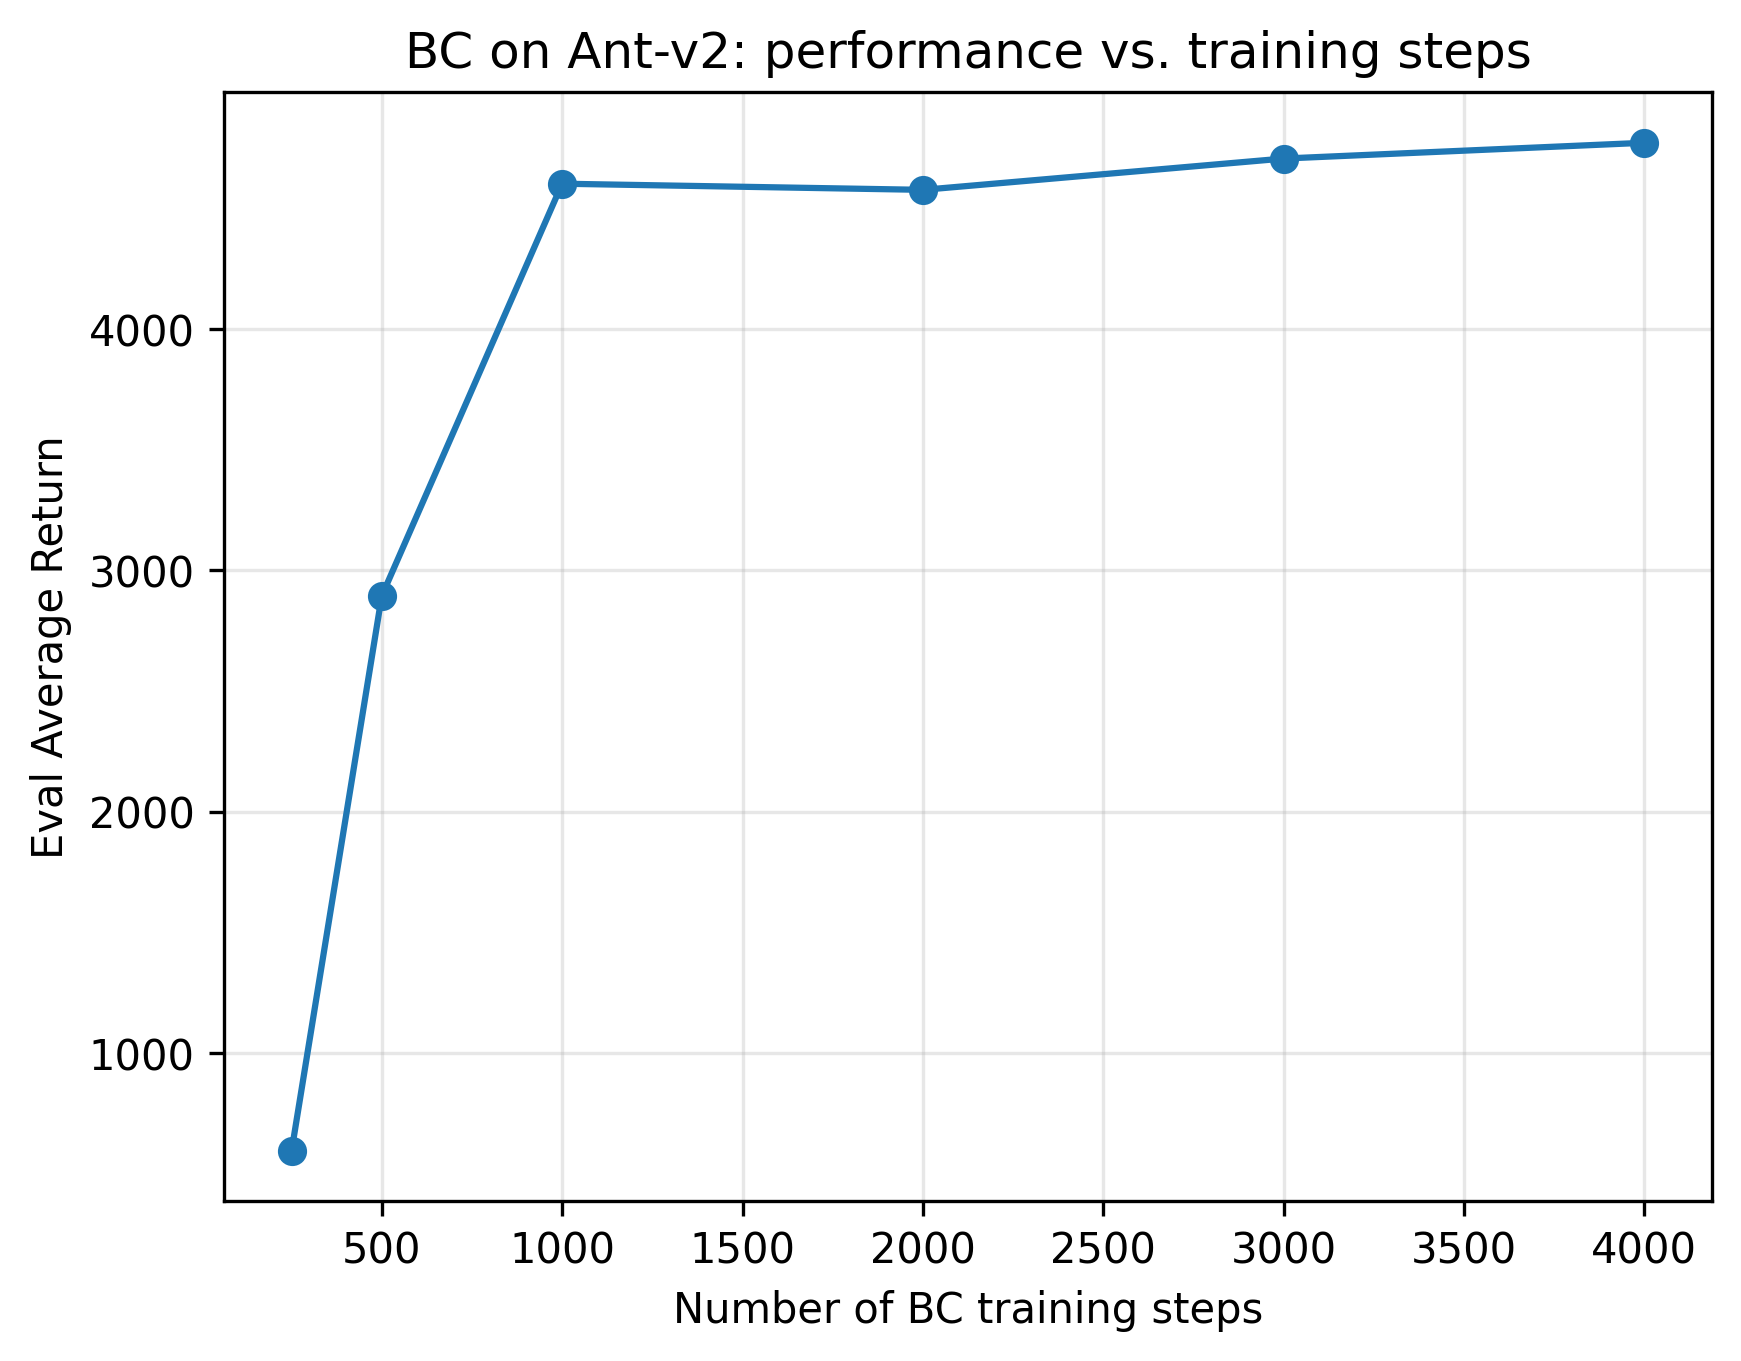
\includegraphics[width=0.5\columnwidth]{data/fig_p4_ant_train_steps.png}
  \caption{Behavioral cloning (BC) performance on \textbf{Ant-v2} as a function of the
  \emph{number of training steps per iteration}. Points show the evaluation
  mean return over at least five rollouts with standard-deviation error bars.
  Increasing the training steps dramatically improves performance from severe
  underfitting (250 steps) to near-expert performance around 3–4k steps, after
  which gains taper off.}
  \label{fig:p4}
\end{figure*}

\# TODO, fill in the \fref{fig:p4}, provide some analysis.


\section{DAgger (5.25 pt)}
\subsection{Part 2 (5.25 pt)}
\# TODO, Report the results for Ant-v2 and [Another Env] in \fref{fig:p5}:
\begin{figure*}[!h]
	\centering
	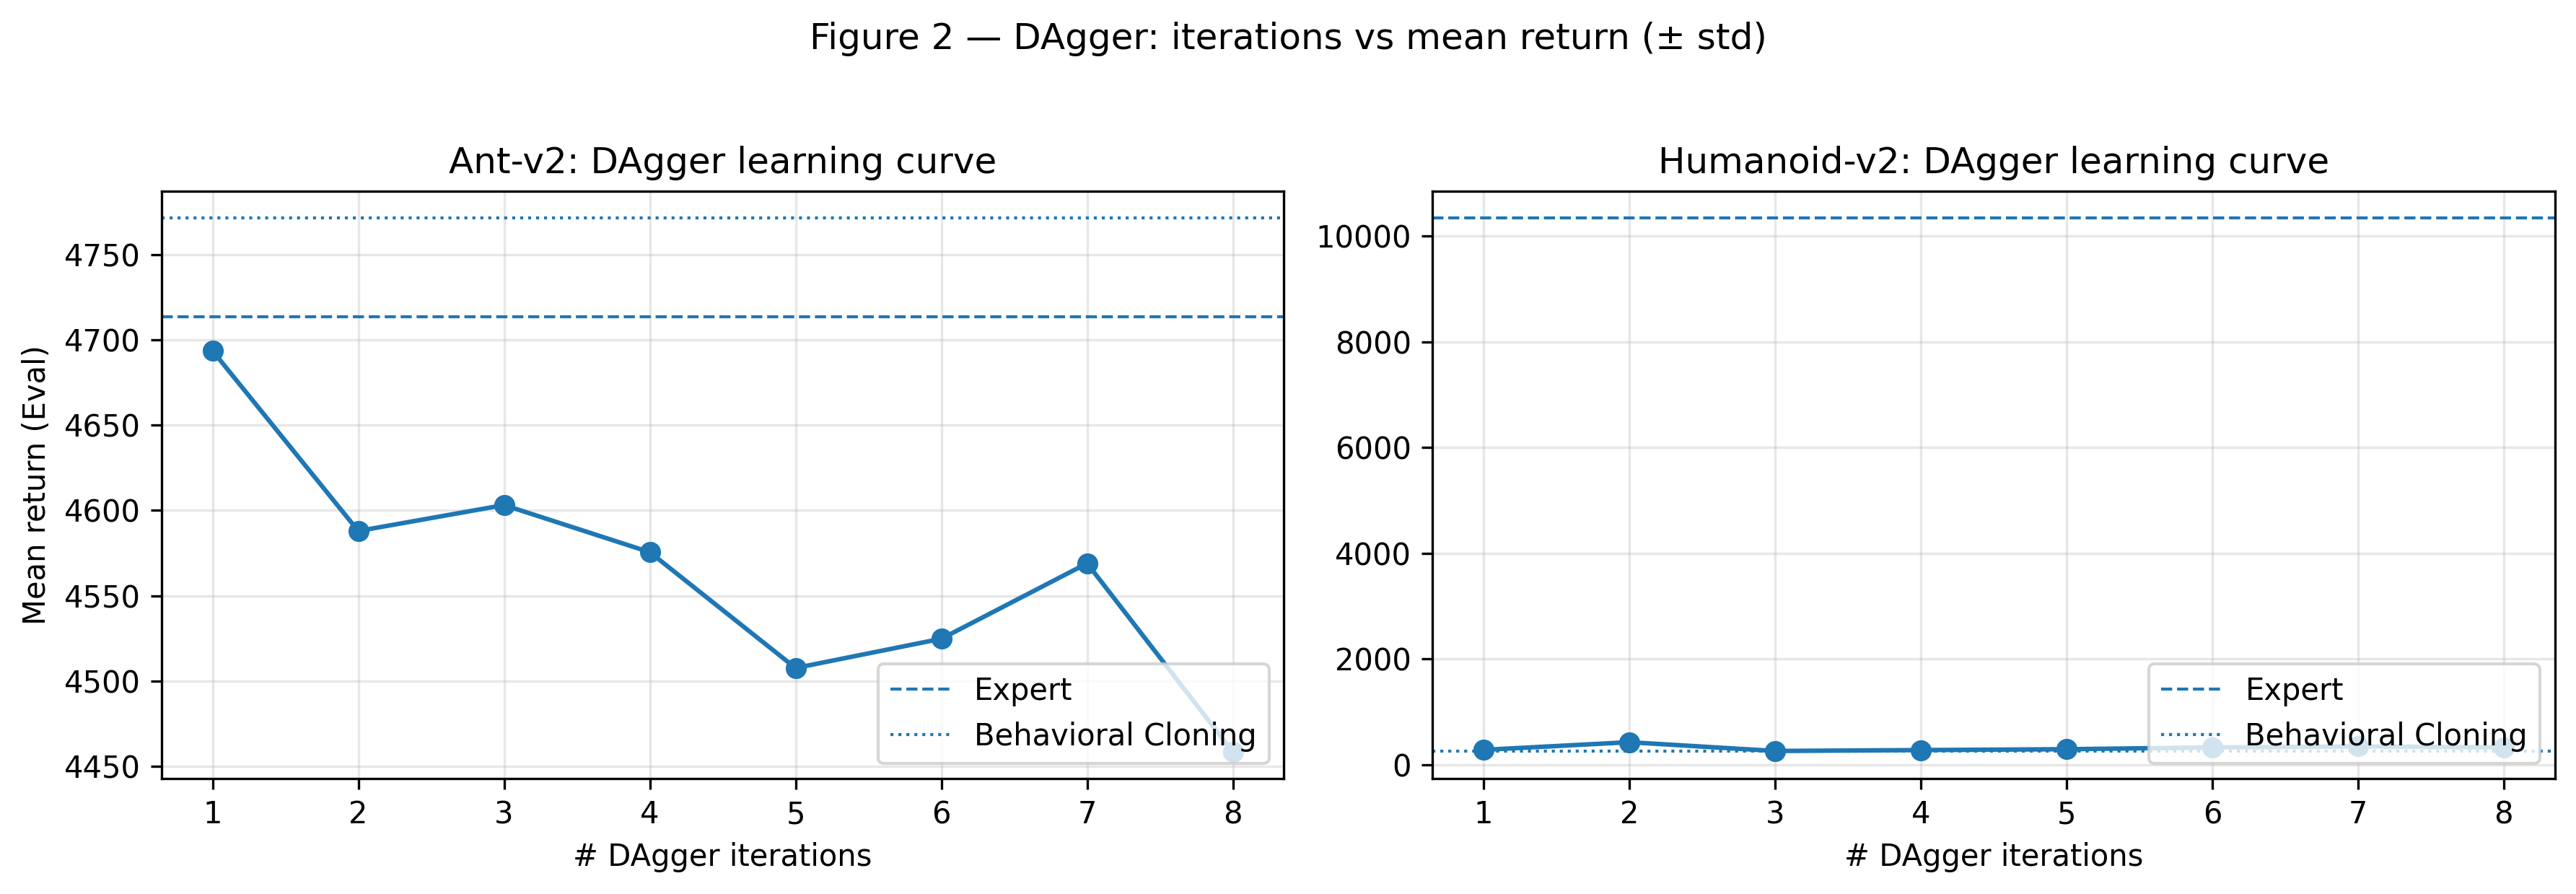
\includegraphics[width=1.0\columnwidth]{data/figure_2_dagger_ant_humanoid.png}
	\caption{DAgger performance on \textbf{Ant-v2} (left) and \textbf{Humanoid-v2} (right).
  Curves plot evaluation mean return versus DAgger iteration, with error bars showing the standard deviation across evaluation rollouts.
  Horizontal dashed/dotted lines show the expert policy and behavioral cloning (BC) baselines, respectively.
  Setup: DAgger used a 3-layer MLP (\texttt{--n\_layers 3}), learning rate $4\times10^{-3}$, 
  evaluation batch size 5000; expert datasets from \texttt{rob831/expert\_data} (Ant-v2 and Humanoid-v2).
  BC baselines were trained with the same learning rate and (for Ant) a 5-layer MLP.}
	\label{fig:p5}
\end{figure*}

\end{document}
